\documentclass[1p]{elsarticle_modified}
%\bibliographystyle{elsarticle-num}

%\usepackage[colorlinks]{hyperref}
%\usepackage{abbrmath_seonhwa} %\Abb, \Ascr, \Acal ,\Abf, \Afrak
\usepackage{amsfonts}
\usepackage{amssymb}
\usepackage{amsmath}
\usepackage{amsthm}
\usepackage{scalefnt}
\usepackage{amsbsy}
\usepackage{kotex}
\usepackage{caption}
\usepackage{subfig}
\usepackage{color}
\usepackage{graphicx}
\usepackage{xcolor} %% white, black, red, green, blue, cyan, magenta, yellow
\usepackage{float}
\usepackage{setspace}
\usepackage{hyperref}

\usepackage{tikz}
\usetikzlibrary{arrows}

\usepackage{multirow}
\usepackage{array} % fixed length table
\usepackage{hhline}

%%%%%%%%%%%%%%%%%%%%%
\makeatletter
\renewcommand*\env@matrix[1][\arraystretch]{%
	\edef\arraystretch{#1}%
	\hskip -\arraycolsep
	\let\@ifnextchar\new@ifnextchar
	\array{*\c@MaxMatrixCols c}}
\makeatother %https://tex.stackexchange.com/questions/14071/how-can-i-increase-the-line-spacing-in-a-matrix
%%%%%%%%%%%%%%%

\usepackage[normalem]{ulem}

\newcommand{\msout}[1]{\ifmmode\text{\sout{\ensuremath{#1}}}\else\sout{#1}\fi}
%SOURCE: \msout is \stkout macro in https://tex.stackexchange.com/questions/20609/strikeout-in-math-mode

\newcommand{\cancel}[1]{
	\ifmmode
	{\color{red}\msout{#1}}
	\else
	{\color{red}\sout{#1}}
	\fi
}

\newcommand{\add}[1]{
	{\color{blue}\uwave{#1}}
}

\newcommand{\replace}[2]{
	\ifmmode
	{\color{red}\msout{#1}}{\color{blue}\uwave{#2}}
	\else
	{\color{red}\sout{#1}}{\color{blue}\uwave{#2}}
	\fi
}

\newcommand{\Sol}{\mathcal{S}} %segment
\newcommand{\D}{D} %diagram
\newcommand{\A}{\mathcal{A}} %arc


%%%%%%%%%%%%%%%%%%%%%%%%%%%%%5 test

\def\sl{\operatorname{\textup{SL}}(2,\Cbb)}
\def\psl{\operatorname{\textup{PSL}}(2,\Cbb)}
\def\quan{\mkern 1mu \triangleright \mkern 1mu}

\theoremstyle{definition}
\newtheorem{thm}{Theorem}[section]
\newtheorem{prop}[thm]{Proposition}
\newtheorem{lem}[thm]{Lemma}
\newtheorem{ques}[thm]{Question}
\newtheorem{cor}[thm]{Corollary}
\newtheorem{defn}[thm]{Definition}
\newtheorem{exam}[thm]{Example}
\newtheorem{rmk}[thm]{Remark}
\newtheorem{alg}[thm]{Algorithm}

\newcommand{\I}{\sqrt{-1}}
\begin{document}

%\begin{frontmatter}
%
%\title{Boundary parabolic representations of knots up to 8 crossings}
%
%%% Group authors per affiliation:
%\author{Yunhi Cho} 
%\address{Department of Mathematics, University of Seoul, Seoul, Korea}
%\ead{yhcho@uos.ac.kr}
%
%
%\author{Seonhwa Kim} %\fnref{s_kim}}
%\address{Center for Geometry and Physics, Institute for Basic Science, Pohang, 37673, Korea}
%\ead{ryeona17@ibs.re.kr}
%
%\author{Hyuk Kim}
%\address{Department of Mathematical Sciences, Seoul National University, Seoul 08826, Korea}
%\ead{hyukkim@snu.ac.kr}
%
%\author{Seokbeom Yoon}
%\address{Department of Mathematical Sciences, Seoul National University, Seoul, 08826,  Korea}
%\ead{sbyoon15@snu.ac.kr}
%
%\begin{abstract}
%We find all boundary parabolic representation of knots up to 8 crossings.
%
%\end{abstract}
%\begin{keyword}
%    \MSC[2010] 57M25 
%\end{keyword}
%
%\end{frontmatter}

%\linenumbers
%\tableofcontents
%
\newcommand\colored[1]{\textcolor{white}{\rule[-0.35ex]{0.8em}{1.4ex}}\kern-0.8em\color{red} #1}%
%\newcommand\colored[1]{\textcolor{white}{ #1}\kern-2.17ex	\textcolor{white}{ #1}\kern-1.81ex	\textcolor{white}{ #1}\kern-2.15ex\color{red}#1	}

{\Large $\underline{12a_{0199}~(K12a_{0199})}$}

\setlength{\tabcolsep}{10pt}
\renewcommand{\arraystretch}{1.6}
\vspace{1cm}\begin{tabular}{m{100pt}>{\centering\arraybackslash}m{274pt}}
\multirow{5}{120pt}{
	\centering
	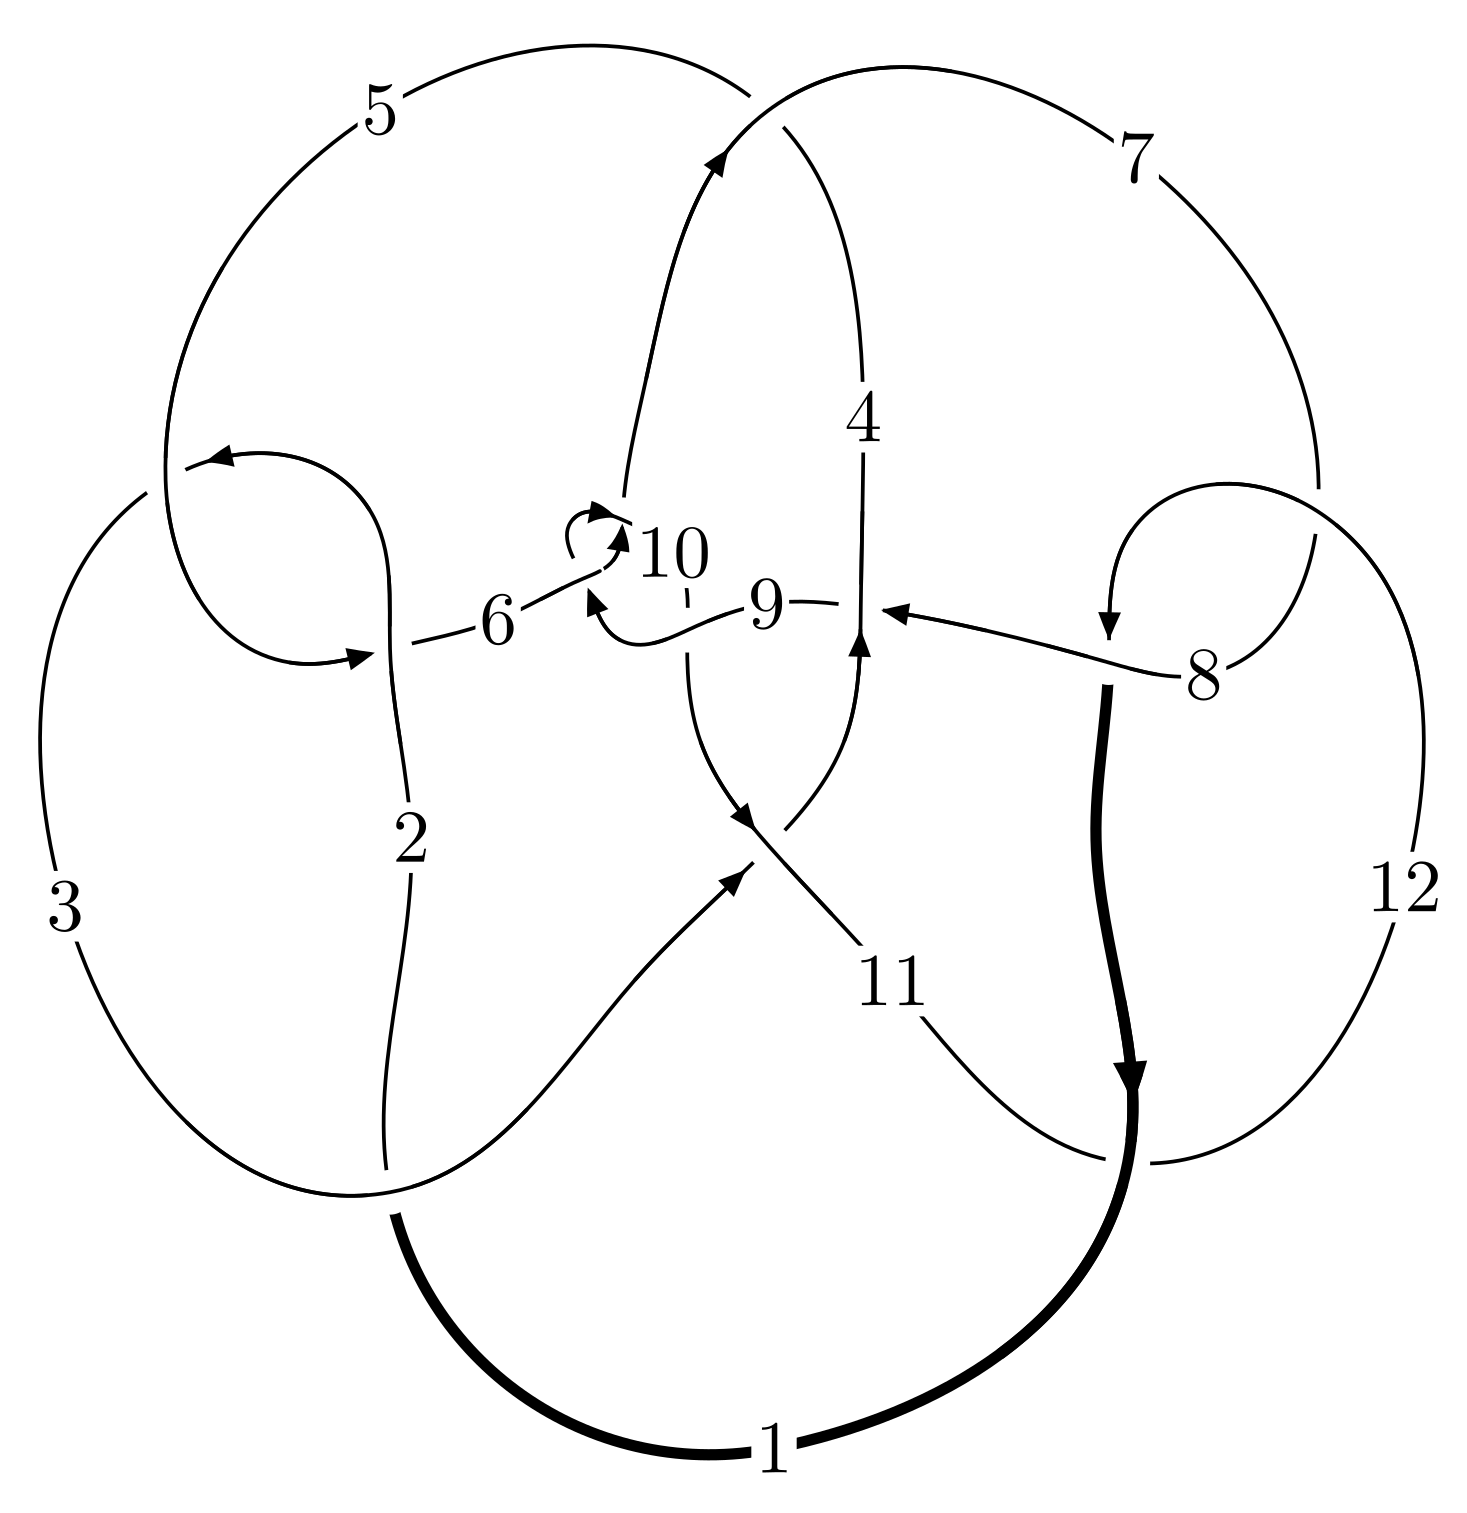
\includegraphics[width=112pt]{../../../GIT/diagram.site/Diagrams/png/1000_12a_0199.png}\\
\ \ \ A knot diagram\footnotemark}&
\allowdisplaybreaks
\textbf{Linearized knot diagam} \\
\cline{2-2}
 &
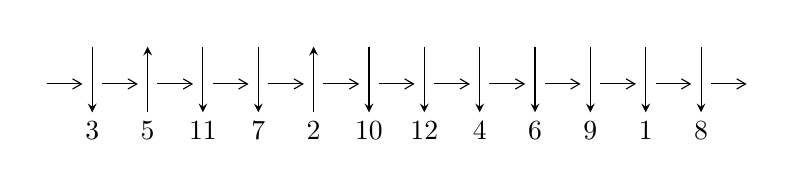
\begin{tikzpicture}[x=20pt, y=17pt]
	% nodes
	\node (C0) at (0, 0) {};
	\node (C1) at (1, 0) {};
	\node (C1U) at (1, +1) {};
	\node (C1D) at (1, -1) {3};

	\node (C2) at (2, 0) {};
	\node (C2U) at (2, +1) {};
	\node (C2D) at (2, -1) {5};

	\node (C3) at (3, 0) {};
	\node (C3U) at (3, +1) {};
	\node (C3D) at (3, -1) {11};

	\node (C4) at (4, 0) {};
	\node (C4U) at (4, +1) {};
	\node (C4D) at (4, -1) {7};

	\node (C5) at (5, 0) {};
	\node (C5U) at (5, +1) {};
	\node (C5D) at (5, -1) {2};

	\node (C6) at (6, 0) {};
	\node (C6U) at (6, +1) {};
	\node (C6D) at (6, -1) {10};

	\node (C7) at (7, 0) {};
	\node (C7U) at (7, +1) {};
	\node (C7D) at (7, -1) {12};

	\node (C8) at (8, 0) {};
	\node (C8U) at (8, +1) {};
	\node (C8D) at (8, -1) {4};

	\node (C9) at (9, 0) {};
	\node (C9U) at (9, +1) {};
	\node (C9D) at (9, -1) {6};

	\node (C10) at (10, 0) {};
	\node (C10U) at (10, +1) {};
	\node (C10D) at (10, -1) {9};

	\node (C11) at (11, 0) {};
	\node (C11U) at (11, +1) {};
	\node (C11D) at (11, -1) {1};

	\node (C12) at (12, 0) {};
	\node (C12U) at (12, +1) {};
	\node (C12D) at (12, -1) {8};
	\node (C13) at (13, 0) {};

	% arrows
	\draw[->,>={angle 60}]
	(C0) edge (C1) (C1) edge (C2) (C2) edge (C3) (C3) edge (C4) (C4) edge (C5) (C5) edge (C6) (C6) edge (C7) (C7) edge (C8) (C8) edge (C9) (C9) edge (C10) (C10) edge (C11) (C11) edge (C12) (C12) edge (C13) ;	\draw[->,>=stealth]
	(C1U) edge (C1D) (C2D) edge (C2U) (C3U) edge (C3D) (C4U) edge (C4D) (C5D) edge (C5U) (C6U) edge (C6D) (C7U) edge (C7D) (C8U) edge (C8D) (C9U) edge (C9D) (C10U) edge (C10D) (C11U) edge (C11D) (C12U) edge (C12D) ;
	\end{tikzpicture} \\
\hhline{~~} \\& 
\textbf{Solving Sequence} \\ \cline{2-2} 
 &
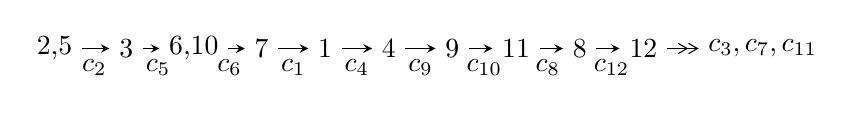
\begin{tikzpicture}[x=23pt, y=7pt]
	% node
	\node (A0) at (-1/8, 0) {2,5};
	\node (A1) at (1, 0) {3};
	\node (A2) at (33/16, 0) {6,10};
	\node (A3) at (25/8, 0) {7};
	\node (A4) at (33/8, 0) {1};
	\node (A5) at (41/8, 0) {4};
	\node (A6) at (49/8, 0) {9};
	\node (A7) at (57/8, 0) {11};
	\node (A8) at (65/8, 0) {8};
	\node (A9) at (73/8, 0) {12};
	\node (C1) at (1/2, -1) {$c_{2}$};
	\node (C2) at (3/2, -1) {$c_{5}$};
	\node (C3) at (21/8, -1) {$c_{6}$};
	\node (C4) at (29/8, -1) {$c_{1}$};
	\node (C5) at (37/8, -1) {$c_{4}$};
	\node (C6) at (45/8, -1) {$c_{9}$};
	\node (C7) at (53/8, -1) {$c_{10}$};
	\node (C8) at (61/8, -1) {$c_{8}$};
	\node (C9) at (69/8, -1) {$c_{12}$};
	\node (A10) at (11, 0) {$c_{3},c_{7},c_{11}$};

	% edge
	\draw[->,>=stealth]	
	(A0) edge (A1) (A1) edge (A2) (A2) edge (A3) (A3) edge (A4) (A4) edge (A5) (A5) edge (A6) (A6) edge (A7) (A7) edge (A8) (A8) edge (A9) ;
	\draw[->>,>={angle 60}]	
	(A9) edge (A10);
\end{tikzpicture} \\ 

\end{tabular} \\

\footnotetext{
The image of knot diagram is generated by the software ``\textbf{Draw programme}" developed by Andrew Bartholomew(\url{http://www.layer8.co.uk/maths/draw/index.htm\#Running-draw}), where we modified some parts for our purpose(\url{https://github.com/CATsTAILs/LinksPainter}).
}\phantom \\ \newline 
\centering \textbf{Ideals for irreducible components\footnotemark of $X_{\text{par}}$} 
 
\begin{align*}
I^u_{1}&=\langle 
-1.05186\times10^{25} u^{29}-1.43266\times10^{24} u^{28}+\cdots+3.83777\times10^{26} b+2.01209\times10^{26},\\
\phantom{I^u_{1}}&\phantom{= \langle  }1.20840\times10^{25} u^{29}+2.78546\times10^{25} u^{28}+\cdots+3.83777\times10^{26} a-1.47083\times10^{27},\;u^{30}+u^{29}+\cdots-136 u+16\rangle \\
I^u_{2}&=\langle 
8301956774068 u^{47} a-1716498814000922 u^{47}+\cdots-18605403975840 a+3278970716047515,\\
\phantom{I^u_{2}}&\phantom{= \langle  }24902419266 u^{47} a+25380336871 u^{47}+\cdots+44502374232 a-179167125090,\\
\phantom{I^u_{2}}&\phantom{= \langle  }u^{48}-2 u^{47}+\cdots+16 u^2+1\rangle \\
I^u_{3}&=\langle 
2 a u+b- a,\;4 a^2-2 a u+u+1,\;u^2+u+1\rangle \\
\\
\end{align*}
\raggedright * 3 irreducible components of $\dim_{\mathbb{C}}=0$, with total 130 representations.\\
\footnotetext{All coefficients of polynomials are rational numbers. But the coefficients are sometimes approximated in decimal forms when there is not enough margin.}
\newpage
\renewcommand{\arraystretch}{1}
\centering \section*{I. $I^u_{1}= \langle -1.05\times10^{25} u^{29}-1.43\times10^{24} u^{28}+\cdots+3.84\times10^{26} b+2.01\times10^{26},\;1.21\times10^{25} u^{29}+2.79\times10^{25} u^{28}+\cdots+3.84\times10^{26} a-1.47\times10^{27},\;u^{30}+u^{29}+\cdots-136 u+16 \rangle$}
\flushleft \textbf{(i) Arc colorings}\\
\begin{tabular}{m{7pt} m{180pt} m{7pt} m{180pt} }
\flushright $a_{2}=$&$\begin{pmatrix}1\\0\end{pmatrix}$ \\
\flushright $a_{5}=$&$\begin{pmatrix}0\\u\end{pmatrix}$ \\
\flushright $a_{3}=$&$\begin{pmatrix}1\\- u^2\end{pmatrix}$ \\
\flushright $a_{6}=$&$\begin{pmatrix}u\\u\end{pmatrix}$ \\
\flushright $a_{10}=$&$\begin{pmatrix}-0.0314870 u^{29}-0.0725802 u^{28}+\cdots-3.16309 u+3.83250\\0.0274082 u^{29}+0.00373306 u^{28}+\cdots+1.51313 u-0.524287\end{pmatrix}$ \\
\flushright $a_{7}=$&$\begin{pmatrix}0.00441977 u^{29}+0.0255666 u^{28}+\cdots-0.244085 u-1.67888\\-0.0228435 u^{29}+0.0213127 u^{28}+\cdots-5.26346 u+0.973918\end{pmatrix}$ \\
\flushright $a_{1}=$&$\begin{pmatrix}u^2+1\\- u^4\end{pmatrix}$ \\
\flushright $a_{4}=$&$\begin{pmatrix}0.00435453 u^{29}+0.00268953 u^{28}+\cdots+1.16324 u+0.264419\\-0.00450085 u^{29}-0.00348346 u^{28}+\cdots+1.15275 u-0.0963126\end{pmatrix}$ \\
\flushright $a_{9}=$&$\begin{pmatrix}-0.0381470 u^{29}-0.0678968 u^{28}+\cdots-1.73655 u+3.55381\\0.0207481 u^{29}+0.00841644 u^{28}+\cdots+2.93967 u-0.802977\end{pmatrix}$ \\
\flushright $a_{11}=$&$\begin{pmatrix}-0.0397231 u^{29}-0.0645166 u^{28}+\cdots-4.17765 u+2.94412\\-0.00367619 u^{29}-0.0461053 u^{28}+\cdots+1.65856 u-0.467412\end{pmatrix}$ \\
\flushright $a_{8}=$&$\begin{pmatrix}-0.0204362 u^{29}-0.0555509 u^{28}+\cdots-0.715574 u+3.27528\\0.0267068 u^{29}-0.0127292 u^{28}+\cdots+6.08279 u-1.17219\end{pmatrix}$ \\
\flushright $a_{12}=$&$\begin{pmatrix}-0.0286036 u^{29}-0.0437086 u^{28}+\cdots-2.32665 u+2.99514\\-0.00925796 u^{29}-0.0455321 u^{28}+\cdots+3.42484 u-0.697592\end{pmatrix}$\\&\end{tabular}
\flushleft \textbf{(ii) Obstruction class $= -1$}\\~\\
\flushleft \textbf{(iii) Cusp Shapes $= -\frac{12790684592978423102182111}{95944166907326703898487264} u^{29}+\frac{24283871709880963319867825}{95944166907326703898487264} u^{28}+\cdots-\frac{443477214659957979551419763}{11993020863415837987310908} u-\frac{42761849795147821338360495}{5996510431707918993655454}$}\\~\\
\newpage\renewcommand{\arraystretch}{1}
\flushleft \textbf{(iv) u-Polynomials at the component}\newline \\
\begin{tabular}{m{50pt}|m{274pt}}
Crossings & \hspace{64pt}u-Polynomials at each crossing \\
\hline $$\begin{aligned}c_{1}\end{aligned}$$&$\begin{aligned}
&u^{30}+11 u^{29}+\cdots-12320 u+256
\end{aligned}$\\
\hline $$\begin{aligned}c_{2},c_{5}\end{aligned}$$&$\begin{aligned}
&u^{30}- u^{29}+\cdots+136 u+16
\end{aligned}$\\
\hline $$\begin{aligned}c_{3},c_{4}\end{aligned}$$&$\begin{aligned}
&16(16 u^{30}-24 u^{29}+\cdots+u+1)
\end{aligned}$\\
\hline $$\begin{aligned}c_{6},c_{7},c_{9}\\c_{12}\end{aligned}$$&$\begin{aligned}
&u^{30}-2 u^{29}+\cdots+3 u-1
\end{aligned}$\\
\hline $$\begin{aligned}c_{8}\end{aligned}$$&$\begin{aligned}
&u^{30}+5 u^{29}+\cdots-9216 u-1024
\end{aligned}$\\
\hline $$\begin{aligned}c_{10},c_{11}\end{aligned}$$&$\begin{aligned}
&u^{30}+16 u^{29}+\cdots+9 u+1
\end{aligned}$\\
\hline
\end{tabular}\\~\\
\newpage\renewcommand{\arraystretch}{1}
\flushleft \textbf{(v) Riley Polynomials at the component}\newline \\
\begin{tabular}{m{50pt}|m{274pt}}
Crossings & \hspace{64pt}Riley Polynomials at each crossing \\
\hline $$\begin{aligned}c_{1}\end{aligned}$$&$\begin{aligned}
&y^{30}+15 y^{29}+\cdots-173031936 y+65536
\end{aligned}$\\
\hline $$\begin{aligned}c_{2},c_{5}\end{aligned}$$&$\begin{aligned}
&y^{30}+11 y^{29}+\cdots-12320 y+256
\end{aligned}$\\
\hline $$\begin{aligned}c_{3},c_{4}\end{aligned}$$&$\begin{aligned}
&256(256 y^{30}+2752 y^{29}+\cdots+y+1)
\end{aligned}$\\
\hline $$\begin{aligned}c_{6},c_{7},c_{9}\\c_{12}\end{aligned}$$&$\begin{aligned}
&y^{30}-16 y^{29}+\cdots-9 y+1
\end{aligned}$\\
\hline $$\begin{aligned}c_{8}\end{aligned}$$&$\begin{aligned}
&y^{30}+5 y^{29}+\cdots+21626880 y+1048576
\end{aligned}$\\
\hline $$\begin{aligned}c_{10},c_{11}\end{aligned}$$&$\begin{aligned}
&y^{30}-48 y^{28}+\cdots+87 y+1
\end{aligned}$\\
\hline
\end{tabular}\\~\\
\newpage\flushleft \textbf{(vi) Complex Volumes and Cusp Shapes}
$$\begin{array}{c|c|c}  
\text{Solutions to }I^u_{1}& \I (\text{vol} + \sqrt{-1}CS) & \text{Cusp shape}\\
 \hline 
\begin{aligned}
u &= \phantom{-}0.513843 + 0.871891 I \\
a &= -0.446146 - 0.725334 I \\
b &= \phantom{-}0.38934 - 2.10569 I\end{aligned}
 & -8.85186 + 2.07542 I & \phantom{-}33.6724 - 61.7857 I \\ \hline\begin{aligned}
u &= \phantom{-}0.513843 - 0.871891 I \\
a &= -0.446146 + 0.725334 I \\
b &= \phantom{-}0.38934 + 2.10569 I\end{aligned}
 & -8.85186 - 2.07542 I & \phantom{-}33.6724 + 61.7857 I \\ \hline\begin{aligned}
u &= -0.355475 + 0.904157 I \\
a &= \phantom{-}0.411047 - 0.455694 I \\
b &= \phantom{-}0.035443 - 0.584835 I\end{aligned}
 & -0.39684 - 1.65663 I & -3.61734 + 2.59404 I \\ \hline\begin{aligned}
u &= -0.355475 - 0.904157 I \\
a &= \phantom{-}0.411047 + 0.455694 I \\
b &= \phantom{-}0.035443 + 0.584835 I\end{aligned}
 & -0.39684 + 1.65663 I & -3.61734 - 2.59404 I \\ \hline\begin{aligned}
u &= \phantom{-}0.886842 + 0.643141 I \\
a &= \phantom{-}0.108219 + 0.207785 I \\
b &= \phantom{-}0.056684 - 0.750111 I\end{aligned}
 & \phantom{-}7.28214 - 1.89713 I & -1.79602 - 0.99400 I \\ \hline\begin{aligned}
u &= \phantom{-}0.886842 - 0.643141 I \\
a &= \phantom{-}0.108219 - 0.207785 I \\
b &= \phantom{-}0.056684 + 0.750111 I\end{aligned}
 & \phantom{-}7.28214 + 1.89713 I & -1.79602 + 0.99400 I \\ \hline\begin{aligned}
u &= -0.270910 + 1.074590 I \\
a &= -1.07328 + 1.52289 I \\
b &= -0.72130 + 2.24404 I\end{aligned}
 & -3.48392 - 0.63227 I & -16.5794 + 0.3609 I \\ \hline\begin{aligned}
u &= -0.270910 - 1.074590 I \\
a &= -1.07328 - 1.52289 I \\
b &= -0.72130 - 2.24404 I\end{aligned}
 & -3.48392 + 0.63227 I & -16.5794 - 0.3609 I \\ \hline\begin{aligned}
u &= \phantom{-}0.989431 + 0.528893 I \\
a &= \phantom{-}2.04634 - 0.16797 I \\
b &= \phantom{-}0.906269 - 0.257371 I\end{aligned}
 & \phantom{-}4.1464 - 13.5352 I & -6.25412 + 8.07209 I \\ \hline\begin{aligned}
u &= \phantom{-}0.989431 - 0.528893 I \\
a &= \phantom{-}2.04634 + 0.16797 I \\
b &= \phantom{-}0.906269 + 0.257371 I\end{aligned}
 & \phantom{-}4.1464 + 13.5352 I & -6.25412 - 8.07209 I\\
 \hline 
 \end{array}$$\newpage$$\begin{array}{c|c|c}  
\text{Solutions to }I^u_{1}& \I (\text{vol} + \sqrt{-1}CS) & \text{Cusp shape}\\
 \hline 
\begin{aligned}
u &= \phantom{-}0.333835 + 1.072850 I \\
a &= \phantom{-}0.15424 - 1.54650 I \\
b &= \phantom{-}0.33154 - 2.61604 I\end{aligned}
 & -8.69259 + 3.42736 I & -19.7102 - 3.7396 I \\ \hline\begin{aligned}
u &= \phantom{-}0.333835 - 1.072850 I \\
a &= \phantom{-}0.15424 + 1.54650 I \\
b &= \phantom{-}0.33154 + 2.61604 I\end{aligned}
 & -8.69259 - 3.42736 I & -19.7102 + 3.7396 I \\ \hline\begin{aligned}
u &= -0.369336 + 1.114300 I \\
a &= \phantom{-}0.386505 - 0.563344 I \\
b &= -0.127883 - 0.862401 I\end{aligned}
 & -0.33657 - 1.57944 I & -6.03935 + 1.36982 I \\ \hline\begin{aligned}
u &= -0.369336 - 1.114300 I \\
a &= \phantom{-}0.386505 + 0.563344 I \\
b &= -0.127883 + 0.862401 I\end{aligned}
 & -0.33657 + 1.57944 I & -6.03935 - 1.36982 I \\ \hline\begin{aligned}
u &= -1.146190 + 0.299068 I \\
a &= \phantom{-}1.55316 + 0.09412 I \\
b &= \phantom{-}0.749359 + 0.445987 I\end{aligned}
 & \phantom{-}4.59032 + 3.09332 I & \phantom{-}1.17313 - 4.12974 I \\ \hline\begin{aligned}
u &= -1.146190 - 0.299068 I \\
a &= \phantom{-}1.55316 - 0.09412 I \\
b &= \phantom{-}0.749359 - 0.445987 I\end{aligned}
 & \phantom{-}4.59032 - 3.09332 I & \phantom{-}1.17313 + 4.12974 I \\ \hline\begin{aligned}
u &= \phantom{-}0.727436 + 1.053530 I \\
a &= -0.047464 + 0.176285 I \\
b &= \phantom{-}0.776365 + 0.265918 I\end{aligned}
 & \phantom{-}6.01261 + 7.86778 I & -3.60910 - 3.95992 I \\ \hline\begin{aligned}
u &= \phantom{-}0.727436 - 1.053530 I \\
a &= -0.047464 - 0.176285 I \\
b &= \phantom{-}0.776365 - 0.265918 I\end{aligned}
 & \phantom{-}6.01261 - 7.86778 I & -3.60910 + 3.95992 I \\ \hline\begin{aligned}
u &= -1.136890 + 0.641709 I \\
a &= -0.623817 + 0.518365 I \\
b &= -0.279528 + 1.274650 I\end{aligned}
 & \phantom{-}4.21761 - 6.91864 I & -0.34998 + 9.53979 I \\ \hline\begin{aligned}
u &= -1.136890 - 0.641709 I \\
a &= -0.623817 - 0.518365 I \\
b &= -0.279528 - 1.274650 I\end{aligned}
 & \phantom{-}4.21761 + 6.91864 I & -0.34998 - 9.53979 I\\
 \hline 
 \end{array}$$\newpage$$\begin{array}{c|c|c}  
\text{Solutions to }I^u_{1}& \I (\text{vol} + \sqrt{-1}CS) & \text{Cusp shape}\\
 \hline 
\begin{aligned}
u &= \phantom{-}0.720787 + 1.140920 I \\
a &= -0.21243 + 2.06553 I \\
b &= -0.22299 + 3.04110 I\end{aligned}
 & \phantom{-}2.2432 + 19.7483 I & -8.5481 - 11.6447 I \\ \hline\begin{aligned}
u &= \phantom{-}0.720787 - 1.140920 I \\
a &= -0.21243 - 2.06553 I \\
b &= -0.22299 - 3.04110 I\end{aligned}
 & \phantom{-}2.2432 - 19.7483 I & -8.5481 + 11.6447 I \\ \hline\begin{aligned}
u &= \phantom{-}0.646093\phantom{ +0.000000I} \\
a &= -1.97921\phantom{ +0.000000I} \\
b &= -0.298708\phantom{ +0.000000I}\end{aligned}
 & -5.53280\phantom{ +0.000000I} & -15.4870\phantom{ +0.000000I} \\ \hline\begin{aligned}
u &= -0.901122 + 1.028260 I \\
a &= -0.918924 - 0.071187 I \\
b &= -0.226436 + 0.036666 I\end{aligned}
 & \phantom{-}3.03751 - 0.25657 I & -1.246747 + 0.314424 I \\ \hline\begin{aligned}
u &= -0.901122 - 1.028260 I \\
a &= -0.918924 + 0.071187 I \\
b &= -0.226436 - 0.036666 I\end{aligned}
 & \phantom{-}3.03751 + 0.25657 I & -1.246747 - 0.314424 I \\ \hline\begin{aligned}
u &= -0.095565 + 1.384150 I \\
a &= \phantom{-}0.39805 + 1.76502 I \\
b &= \phantom{-}0.02520 + 2.54016 I\end{aligned}
 & -3.39765 - 10.83270 I & -11.6079 + 10.7508 I \\ \hline\begin{aligned}
u &= -0.095565 - 1.384150 I \\
a &= \phantom{-}0.39805 - 1.76502 I \\
b &= \phantom{-}0.02520 - 2.54016 I\end{aligned}
 & -3.39765 + 10.83270 I & -11.6079 - 10.7508 I \\ \hline\begin{aligned}
u &= -0.78951 + 1.26116 I \\
a &= -0.08887 - 1.76517 I \\
b &= -0.07406 - 2.52275 I\end{aligned}
 & \phantom{-}1.73617 - 9.98872 I & -5.29929 + 12.58752 I \\ \hline\begin{aligned}
u &= -0.78951 - 1.26116 I \\
a &= -0.08887 + 1.76517 I \\
b &= -0.07406 + 2.52275 I\end{aligned}
 & \phantom{-}1.73617 + 9.98872 I & -5.29929 - 12.58752 I \\ \hline\begin{aligned}
u &= \phantom{-}0.139554\phantom{ +0.000000I} \\
a &= \phantom{-}3.43594\phantom{ +0.000000I} \\
b &= -0.437309\phantom{ +0.000000I}\end{aligned}
 & -0.810611\phantom{ +0.000000I} & -12.3890\phantom{ +0.000000I}\\
 \hline 
 \end{array}$$\newpage\newpage\renewcommand{\arraystretch}{1}
\centering \section*{II. $I^u_{2}= \langle 8.30\times10^{12} a u^{47}-1.72\times10^{15} u^{47}+\cdots-1.86\times10^{13} a+3.28\times10^{15},\;2.49\times10^{10} a u^{47}+2.54\times10^{10} u^{47}+\cdots+4.45\times10^{10} a-1.79\times10^{11},\;u^{48}-2 u^{47}+\cdots+16 u^2+1 \rangle$}
\flushleft \textbf{(i) Arc colorings}\\
\begin{tabular}{m{7pt} m{180pt} m{7pt} m{180pt} }
\flushright $a_{2}=$&$\begin{pmatrix}1\\0\end{pmatrix}$ \\
\flushright $a_{5}=$&$\begin{pmatrix}0\\u\end{pmatrix}$ \\
\flushright $a_{3}=$&$\begin{pmatrix}1\\- u^2\end{pmatrix}$ \\
\flushright $a_{6}=$&$\begin{pmatrix}u\\u\end{pmatrix}$ \\
\flushright $a_{10}=$&$\begin{pmatrix}a\\-0.00768508 a u^{47}+1.58895 u^{47}+\cdots+0.0172229 a-3.03533\end{pmatrix}$ \\
\flushright $a_{7}=$&$\begin{pmatrix}0.913597 a u^{47}-1.12318 u^{47}+\cdots-3.05186 a-4.32727\\1.69606 a u^{47}-2.47177 u^{47}+\cdots+1.67376 a+0.0264682\end{pmatrix}$ \\
\flushright $a_{1}=$&$\begin{pmatrix}u^2+1\\- u^4\end{pmatrix}$ \\
\flushright $a_{4}=$&$\begin{pmatrix}-0.895600 a u^{47}+1.48267 u^{47}+\cdots+1.88285 a+10.0601\\-0.805141 a u^{47}+0.416548 u^{47}+\cdots-0.739690 a+0.986881\end{pmatrix}$ \\
\flushright $a_{9}=$&$\begin{pmatrix}0.222411 a u^{47}+0.533718 u^{47}+\cdots+1.07881 a-1.01638\\0.214726 a u^{47}+2.12267 u^{47}+\cdots+0.0960309 a-4.05170\end{pmatrix}$ \\
\flushright $a_{11}=$&$\begin{pmatrix}2.20533 a u^{47}-1.56856 u^{47}+\cdots-4.28442 a-7.99229\\2.65700 a u^{47}-0.108542 u^{47}+\cdots-0.172526 a-3.38343\end{pmatrix}$ \\
\flushright $a_{8}=$&$\begin{pmatrix}0.391848 a u^{47}+0.489312 u^{47}+\cdots+0.237285 a-5.57041\\0.391848 a u^{47}+2.93394 u^{47}+\cdots+0.237285 a-4.59756\end{pmatrix}$ \\
\flushright $a_{12}=$&$\begin{pmatrix}-1.89258 a u^{47}-1.52697 u^{47}+\cdots-0.347615 a-7.31396\\-1.43205 a u^{47}+1.08570 u^{47}+\cdots+2.37872 a-4.96729\end{pmatrix}$\\&\end{tabular}
\flushleft \textbf{(ii) Obstruction class $= -1$}\\~\\
\flushleft \textbf{(iii) Cusp Shapes $= -\frac{17136040638}{3523750753} u^{47}+\frac{40416089808}{3523750753} u^{46}+\cdots-\frac{10188595612}{3523750753} u-\frac{39541667460}{3523750753}$}\\~\\
\newpage\renewcommand{\arraystretch}{1}
\flushleft \textbf{(iv) u-Polynomials at the component}\newline \\
\begin{tabular}{m{50pt}|m{274pt}}
Crossings & \hspace{64pt}u-Polynomials at each crossing \\
\hline $$\begin{aligned}c_{1}\end{aligned}$$&$\begin{aligned}
&(u^{48}+18 u^{47}+\cdots+32 u+1)^{2}
\end{aligned}$\\
\hline $$\begin{aligned}c_{2},c_{5}\end{aligned}$$&$\begin{aligned}
&(u^{48}+2 u^{47}+\cdots+16 u^2+1)^{2}
\end{aligned}$\\
\hline $$\begin{aligned}c_{3},c_{4}\end{aligned}$$&$\begin{aligned}
&u^{96}-9 u^{95}+\cdots+130810298 u+122183483
\end{aligned}$\\
\hline $$\begin{aligned}c_{6},c_{7},c_{9}\\c_{12}\end{aligned}$$&$\begin{aligned}
&u^{96}+5 u^{95}+\cdots+2 u+1
\end{aligned}$\\
\hline $$\begin{aligned}c_{8}\end{aligned}$$&$\begin{aligned}
&(u^{48}-2 u^{47}+\cdots+2 u+1)^{2}
\end{aligned}$\\
\hline $$\begin{aligned}c_{10},c_{11}\end{aligned}$$&$\begin{aligned}
&u^{96}+37 u^{95}+\cdots+408 u^3+1
\end{aligned}$\\
\hline
\end{tabular}\\~\\
\newpage\renewcommand{\arraystretch}{1}
\flushleft \textbf{(v) Riley Polynomials at the component}\newline \\
\begin{tabular}{m{50pt}|m{274pt}}
Crossings & \hspace{64pt}Riley Polynomials at each crossing \\
\hline $$\begin{aligned}c_{1}\end{aligned}$$&$\begin{aligned}
&(y^{48}+26 y^{47}+\cdots-264 y+1)^{2}
\end{aligned}$\\
\hline $$\begin{aligned}c_{2},c_{5}\end{aligned}$$&$\begin{aligned}
&(y^{48}+18 y^{47}+\cdots+32 y+1)^{2}
\end{aligned}$\\
\hline $$\begin{aligned}c_{3},c_{4}\end{aligned}$$&$\begin{aligned}
&y^{96}+47 y^{95}+\cdots+239047203594444768 y+14928803518011289
\end{aligned}$\\
\hline $$\begin{aligned}c_{6},c_{7},c_{9}\\c_{12}\end{aligned}$$&$\begin{aligned}
&y^{96}-37 y^{95}+\cdots-408 y^3+1
\end{aligned}$\\
\hline $$\begin{aligned}c_{8}\end{aligned}$$&$\begin{aligned}
&(y^{48}+10 y^{47}+\cdots+20 y+1)^{2}
\end{aligned}$\\
\hline $$\begin{aligned}c_{10},c_{11}\end{aligned}$$&$\begin{aligned}
&y^{96}+43 y^{95}+\cdots+2144 y^2+1
\end{aligned}$\\
\hline
\end{tabular}\\~\\
\newpage\flushleft \textbf{(vi) Complex Volumes and Cusp Shapes}
$$\begin{array}{c|c|c}  
\text{Solutions to }I^u_{2}& \I (\text{vol} + \sqrt{-1}CS) & \text{Cusp shape}\\
 \hline 
\begin{aligned}
u &= -0.484781 + 0.850953 I \\
a &= -3.37504 + 5.83345 I \\
b &= -3.33055 + 4.82375 I\end{aligned}
 & -0.02738 - 1.96363 I & \phantom{-}2.8944 + 51.2708 I \\ \hline\begin{aligned}
u &= -0.484781 + 0.850953 I \\
a &= \phantom{-}0.20739 - 7.60050 I \\
b &= -0.64315 - 8.14498 I\end{aligned}
 & -0.02738 - 1.96363 I & \phantom{-}2.8944 + 51.2708 I \\ \hline\begin{aligned}
u &= -0.484781 - 0.850953 I \\
a &= -3.37504 - 5.83345 I \\
b &= -3.33055 - 4.82375 I\end{aligned}
 & -0.02738 + 1.96363 I & \phantom{-}2.8944 - 51.2708 I \\ \hline\begin{aligned}
u &= -0.484781 - 0.850953 I \\
a &= \phantom{-}0.20739 + 7.60050 I \\
b &= -0.64315 + 8.14498 I\end{aligned}
 & -0.02738 + 1.96363 I & \phantom{-}2.8944 - 51.2708 I \\ \hline\begin{aligned}
u &= \phantom{-}0.097067 + 1.022650 I \\
a &= -0.406779 + 0.448418 I \\
b &= \phantom{-}0.253041 + 0.768046 I\end{aligned}
 & -3.99758 + 0.49161 I & -13.81533 - 0.65955 I \\ \hline\begin{aligned}
u &= \phantom{-}0.097067 + 1.022650 I \\
a &= -0.72794 + 1.49597 I \\
b &= -0.61571 + 2.57000 I\end{aligned}
 & -3.99758 + 0.49161 I & -13.81533 - 0.65955 I \\ \hline\begin{aligned}
u &= \phantom{-}0.097067 - 1.022650 I \\
a &= -0.406779 - 0.448418 I \\
b &= \phantom{-}0.253041 - 0.768046 I\end{aligned}
 & -3.99758 - 0.49161 I & -13.81533 + 0.65955 I \\ \hline\begin{aligned}
u &= \phantom{-}0.097067 - 1.022650 I \\
a &= -0.72794 - 1.49597 I \\
b &= -0.61571 - 2.57000 I\end{aligned}
 & -3.99758 - 0.49161 I & -13.81533 + 0.65955 I \\ \hline\begin{aligned}
u &= \phantom{-}0.716038 + 0.740578 I \\
a &= -1.58024 + 0.04054 I \\
b &= -0.327130 - 0.220538 I\end{aligned}
 & \phantom{-}4.67401 - 3.43632 I & -1.94110 + 3.09138 I \\ \hline\begin{aligned}
u &= \phantom{-}0.716038 + 0.740578 I \\
a &= \phantom{-}0.292211 - 0.016004 I \\
b &= -0.626333 - 0.371523 I\end{aligned}
 & \phantom{-}4.67401 - 3.43632 I & -1.94110 + 3.09138 I\\
 \hline 
 \end{array}$$\newpage$$\begin{array}{c|c|c}  
\text{Solutions to }I^u_{2}& \I (\text{vol} + \sqrt{-1}CS) & \text{Cusp shape}\\
 \hline 
\begin{aligned}
u &= \phantom{-}0.716038 - 0.740578 I \\
a &= -1.58024 - 0.04054 I \\
b &= -0.327130 + 0.220538 I\end{aligned}
 & \phantom{-}4.67401 + 3.43632 I & -1.94110 - 3.09138 I \\ \hline\begin{aligned}
u &= \phantom{-}0.716038 - 0.740578 I \\
a &= \phantom{-}0.292211 + 0.016004 I \\
b &= -0.626333 + 0.371523 I\end{aligned}
 & \phantom{-}4.67401 + 3.43632 I & -1.94110 - 3.09138 I \\ \hline\begin{aligned}
u &= -0.685446 + 0.778575 I \\
a &= -0.298304 - 0.757635 I \\
b &= -0.444479 - 0.452774 I\end{aligned}
 & \phantom{-}1.43924 - 0.31691 I & -6.77030 + 0.34002 I \\ \hline\begin{aligned}
u &= -0.685446 + 0.778575 I \\
a &= -1.15899 - 1.04942 I \\
b &= -0.234179 - 0.846072 I\end{aligned}
 & \phantom{-}1.43924 - 0.31691 I & -6.77030 + 0.34002 I \\ \hline\begin{aligned}
u &= -0.685446 - 0.778575 I \\
a &= -0.298304 + 0.757635 I \\
b &= -0.444479 + 0.452774 I\end{aligned}
 & \phantom{-}1.43924 + 0.31691 I & -6.77030 - 0.34002 I \\ \hline\begin{aligned}
u &= -0.685446 - 0.778575 I \\
a &= -1.15899 + 1.04942 I \\
b &= -0.234179 + 0.846072 I\end{aligned}
 & \phantom{-}1.43924 + 0.31691 I & -6.77030 - 0.34002 I \\ \hline\begin{aligned}
u &= \phantom{-}0.636609 + 0.849934 I \\
a &= \phantom{-}0.078084 + 1.162150 I \\
b &= -0.09338 + 2.45454 I\end{aligned}
 & \phantom{-}2.20823 + 2.48736 I & -1.52867 - 3.91872 I \\ \hline\begin{aligned}
u &= \phantom{-}0.636609 + 0.849934 I \\
a &= \phantom{-}1.311060 + 0.127836 I \\
b &= \phantom{-}0.091787 + 0.556421 I\end{aligned}
 & \phantom{-}2.20823 + 2.48736 I & -1.52867 - 3.91872 I \\ \hline\begin{aligned}
u &= \phantom{-}0.636609 - 0.849934 I \\
a &= \phantom{-}0.078084 - 1.162150 I \\
b &= -0.09338 - 2.45454 I\end{aligned}
 & \phantom{-}2.20823 - 2.48736 I & -1.52867 + 3.91872 I \\ \hline\begin{aligned}
u &= \phantom{-}0.636609 - 0.849934 I \\
a &= \phantom{-}1.311060 - 0.127836 I \\
b &= \phantom{-}0.091787 - 0.556421 I\end{aligned}
 & \phantom{-}2.20823 - 2.48736 I & -1.52867 + 3.91872 I\\
 \hline 
 \end{array}$$\newpage$$\begin{array}{c|c|c}  
\text{Solutions to }I^u_{2}& \I (\text{vol} + \sqrt{-1}CS) & \text{Cusp shape}\\
 \hline 
\begin{aligned}
u &= \phantom{-}0.936905 + 0.579477 I \\
a &= -0.055387 - 0.251475 I \\
b &= -0.074157 + 0.690139 I\end{aligned}
 & \phantom{-}5.72343 - 7.74189 I & -4.00692 + 3.57032 I \\ \hline\begin{aligned}
u &= \phantom{-}0.936905 + 0.579477 I \\
a &= -1.97766 + 0.12581 I \\
b &= -0.810338 + 0.148751 I\end{aligned}
 & \phantom{-}5.72343 - 7.74189 I & -4.00692 + 3.57032 I \\ \hline\begin{aligned}
u &= \phantom{-}0.936905 - 0.579477 I \\
a &= -0.055387 + 0.251475 I \\
b &= -0.074157 - 0.690139 I\end{aligned}
 & \phantom{-}5.72343 + 7.74189 I & -4.00692 - 3.57032 I \\ \hline\begin{aligned}
u &= \phantom{-}0.936905 - 0.579477 I \\
a &= -1.97766 - 0.12581 I \\
b &= -0.810338 - 0.148751 I\end{aligned}
 & \phantom{-}5.72343 + 7.74189 I & -4.00692 - 3.57032 I \\ \hline\begin{aligned}
u &= \phantom{-}0.717956 + 0.851849 I \\
a &= \phantom{-}0.251023 - 0.019875 I \\
b &= -0.076809 - 0.959910 I\end{aligned}
 & \phantom{-}6.27413 + 2.73487 I & \phantom{-0.000000 } 0. - 3.17064 I \\ \hline\begin{aligned}
u &= \phantom{-}0.717956 + 0.851849 I \\
a &= -0.220056 + 0.082656 I \\
b &= \phantom{-}0.693660 + 0.338468 I\end{aligned}
 & \phantom{-}6.27413 + 2.73487 I & \phantom{-0.000000 } 0. - 3.17064 I \\ \hline\begin{aligned}
u &= \phantom{-}0.717956 - 0.851849 I \\
a &= \phantom{-}0.251023 + 0.019875 I \\
b &= -0.076809 + 0.959910 I\end{aligned}
 & \phantom{-}6.27413 - 2.73487 I & \phantom{-0.000000 -}0. + 3.17064 I \\ \hline\begin{aligned}
u &= \phantom{-}0.717956 - 0.851849 I \\
a &= -0.220056 - 0.082656 I \\
b &= \phantom{-}0.693660 - 0.338468 I\end{aligned}
 & \phantom{-}6.27413 - 2.73487 I & \phantom{-0.000000 -}0. + 3.17064 I \\ \hline\begin{aligned}
u &= -0.684569 + 0.885432 I \\
a &= \phantom{-}0.497504 + 0.678613 I \\
b &= \phantom{-}0.594605 + 0.365341 I\end{aligned}
 & \phantom{-}1.11254 - 4.96052 I & -8.00000 + 5.40900 I \\ \hline\begin{aligned}
u &= -0.684569 + 0.885432 I \\
a &= \phantom{-}1.10653 + 0.94980 I \\
b &= \phantom{-}1.18189 + 1.90242 I\end{aligned}
 & \phantom{-}1.11254 - 4.96052 I & -8.00000 + 5.40900 I\\
 \hline 
 \end{array}$$\newpage$$\begin{array}{c|c|c}  
\text{Solutions to }I^u_{2}& \I (\text{vol} + \sqrt{-1}CS) & \text{Cusp shape}\\
 \hline 
\begin{aligned}
u &= -0.684569 - 0.885432 I \\
a &= \phantom{-}0.497504 - 0.678613 I \\
b &= \phantom{-}0.594605 - 0.365341 I\end{aligned}
 & \phantom{-}1.11254 + 4.96052 I & -8.00000 - 5.40900 I \\ \hline\begin{aligned}
u &= -0.684569 - 0.885432 I \\
a &= \phantom{-}1.10653 - 0.94980 I \\
b &= \phantom{-}1.18189 - 1.90242 I\end{aligned}
 & \phantom{-}1.11254 + 4.96052 I & -8.00000 - 5.40900 I \\ \hline\begin{aligned}
u &= -0.420414 + 0.772149 I \\
a &= \phantom{-}3.55803 + 1.71143 I \\
b &= \phantom{-}2.51087 + 1.16971 I\end{aligned}
 & -0.14530 + 2.51169 I & -9.91381 + 1.94946 I \\ \hline\begin{aligned}
u &= -0.420414 + 0.772149 I \\
a &= -2.15258 + 3.37249 I \\
b &= -1.24231 + 4.05910 I\end{aligned}
 & -0.14530 + 2.51169 I & -9.91381 + 1.94946 I \\ \hline\begin{aligned}
u &= -0.420414 - 0.772149 I \\
a &= \phantom{-}3.55803 - 1.71143 I \\
b &= \phantom{-}2.51087 - 1.16971 I\end{aligned}
 & -0.14530 - 2.51169 I & -9.91381 - 1.94946 I \\ \hline\begin{aligned}
u &= -0.420414 - 0.772149 I \\
a &= -2.15258 - 3.37249 I \\
b &= -1.24231 - 4.05910 I\end{aligned}
 & -0.14530 - 2.51169 I & -9.91381 - 1.94946 I \\ \hline\begin{aligned}
u &= \phantom{-}0.733465 + 0.467600 I \\
a &= -1.65111 - 0.38305 I \\
b &= -0.445586 - 1.014770 I\end{aligned}
 & -0.96653 - 6.30841 I & -9.45390 + 5.38910 I \\ \hline\begin{aligned}
u &= \phantom{-}0.733465 + 0.467600 I \\
a &= \phantom{-}1.86018 - 0.33304 I \\
b &= \phantom{-}0.410288 - 0.363694 I\end{aligned}
 & -0.96653 - 6.30841 I & -9.45390 + 5.38910 I \\ \hline\begin{aligned}
u &= \phantom{-}0.733465 - 0.467600 I \\
a &= -1.65111 + 0.38305 I \\
b &= -0.445586 + 1.014770 I\end{aligned}
 & -0.96653 + 6.30841 I & -9.45390 - 5.38910 I \\ \hline\begin{aligned}
u &= \phantom{-}0.733465 - 0.467600 I \\
a &= \phantom{-}1.86018 + 0.33304 I \\
b &= \phantom{-}0.410288 + 0.363694 I\end{aligned}
 & -0.96653 + 6.30841 I & -9.45390 - 5.38910 I\\
 \hline 
 \end{array}$$\newpage$$\begin{array}{c|c|c}  
\text{Solutions to }I^u_{2}& \I (\text{vol} + \sqrt{-1}CS) & \text{Cusp shape}\\
 \hline 
\begin{aligned}
u &= \phantom{-}0.605495 + 0.621445 I \\
a &= \phantom{-}1.241810 + 0.446110 I \\
b &= \phantom{-}0.123749 + 1.329770 I\end{aligned}
 & \phantom{-}0.278716 - 0.472036 I & -6.31074 + 2.15424 I \\ \hline\begin{aligned}
u &= \phantom{-}0.605495 + 0.621445 I \\
a &= -0.463331 - 0.287948 I \\
b &= -0.267791 + 0.963683 I\end{aligned}
 & \phantom{-}0.278716 - 0.472036 I & -6.31074 + 2.15424 I \\ \hline\begin{aligned}
u &= \phantom{-}0.605495 - 0.621445 I \\
a &= \phantom{-}1.241810 - 0.446110 I \\
b &= \phantom{-}0.123749 - 1.329770 I\end{aligned}
 & \phantom{-}0.278716 + 0.472036 I & -6.31074 - 2.15424 I \\ \hline\begin{aligned}
u &= \phantom{-}0.605495 - 0.621445 I \\
a &= -0.463331 + 0.287948 I \\
b &= -0.267791 - 0.963683 I\end{aligned}
 & \phantom{-}0.278716 + 0.472036 I & -6.31074 - 2.15424 I \\ \hline\begin{aligned}
u &= -0.490818 + 1.023000 I \\
a &= \phantom{-}0.994900 - 0.202633 I \\
b &= \phantom{-}0.826814 - 0.594067 I\end{aligned}
 & -0.41863 - 1.44578 I & -8.00000 - 1.12617 I \\ \hline\begin{aligned}
u &= -0.490818 + 1.023000 I \\
a &= -0.116576 - 0.595943 I \\
b &= -0.743474 - 0.981271 I\end{aligned}
 & -0.41863 - 1.44578 I & -8.00000 - 1.12617 I \\ \hline\begin{aligned}
u &= -0.490818 - 1.023000 I \\
a &= \phantom{-}0.994900 + 0.202633 I \\
b &= \phantom{-}0.826814 + 0.594067 I\end{aligned}
 & -0.41863 + 1.44578 I & -8.00000 + 1.12617 I \\ \hline\begin{aligned}
u &= -0.490818 - 1.023000 I \\
a &= -0.116576 + 0.595943 I \\
b &= -0.743474 + 0.981271 I\end{aligned}
 & -0.41863 + 1.44578 I & -8.00000 + 1.12617 I \\ \hline\begin{aligned}
u &= \phantom{-}0.679611 + 0.941578 I \\
a &= \phantom{-}0.01271 - 1.46261 I \\
b &= \phantom{-}0.11344 - 2.62787 I\end{aligned}
 & \phantom{-}4.06736 + 8.78436 I & -3.69204 - 9.06876 I \\ \hline\begin{aligned}
u &= \phantom{-}0.679611 + 0.941578 I \\
a &= -0.239559 + 0.117695 I \\
b &= \phantom{-}0.175598 + 0.973145 I\end{aligned}
 & \phantom{-}4.06736 + 8.78436 I & -3.69204 - 9.06876 I\\
 \hline 
 \end{array}$$\newpage$$\begin{array}{c|c|c}  
\text{Solutions to }I^u_{2}& \I (\text{vol} + \sqrt{-1}CS) & \text{Cusp shape}\\
 \hline 
\begin{aligned}
u &= \phantom{-}0.679611 - 0.941578 I \\
a &= \phantom{-}0.01271 + 1.46261 I \\
b &= \phantom{-}0.11344 + 2.62787 I\end{aligned}
 & \phantom{-}4.06736 - 8.78436 I & -3.69204 + 9.06876 I \\ \hline\begin{aligned}
u &= \phantom{-}0.679611 - 0.941578 I \\
a &= -0.239559 - 0.117695 I \\
b &= \phantom{-}0.175598 - 0.973145 I\end{aligned}
 & \phantom{-}4.06736 - 8.78436 I & -3.69204 + 9.06876 I \\ \hline\begin{aligned}
u &= \phantom{-}0.618516 + 0.996648 I \\
a &= \phantom{-}0.70483 + 1.36867 I \\
b &= \phantom{-}0.13252 + 2.33095 I\end{aligned}
 & -0.83388 + 5.37086 I & -8.00000 - 6.82742 I \\ \hline\begin{aligned}
u &= \phantom{-}0.618516 + 0.996648 I \\
a &= \phantom{-}0.155618 - 0.259413 I \\
b &= -0.791151 - 0.314501 I\end{aligned}
 & -0.83388 + 5.37086 I & -8.00000 - 6.82742 I \\ \hline\begin{aligned}
u &= \phantom{-}0.618516 - 0.996648 I \\
a &= \phantom{-}0.70483 - 1.36867 I \\
b &= \phantom{-}0.13252 - 2.33095 I\end{aligned}
 & -0.83388 - 5.37086 I & -8.00000 + 6.82742 I \\ \hline\begin{aligned}
u &= \phantom{-}0.618516 - 0.996648 I \\
a &= \phantom{-}0.155618 + 0.259413 I \\
b &= -0.791151 + 0.314501 I\end{aligned}
 & -0.83388 - 5.37086 I & -8.00000 + 6.82742 I \\ \hline\begin{aligned}
u &= \phantom{-}0.092633 + 1.183130 I \\
a &= \phantom{-}0.407430 + 1.310510 I \\
b &= -0.13398 + 2.18038 I\end{aligned}
 & -6.20332 - 4.21770 I & -16.5470 + 3.6832 I \\ \hline\begin{aligned}
u &= \phantom{-}0.092633 + 1.183130 I \\
a &= \phantom{-}0.70859 - 1.82338 I \\
b &= \phantom{-}0.66013 - 2.74184 I\end{aligned}
 & -6.20332 - 4.21770 I & -16.5470 + 3.6832 I \\ \hline\begin{aligned}
u &= \phantom{-}0.092633 - 1.183130 I \\
a &= \phantom{-}0.407430 - 1.310510 I \\
b &= -0.13398 - 2.18038 I\end{aligned}
 & -6.20332 + 4.21770 I & -16.5470 - 3.6832 I \\ \hline\begin{aligned}
u &= \phantom{-}0.092633 - 1.183130 I \\
a &= \phantom{-}0.70859 + 1.82338 I \\
b &= \phantom{-}0.66013 + 2.74184 I\end{aligned}
 & -6.20332 + 4.21770 I & -16.5470 - 3.6832 I\\
 \hline 
 \end{array}$$\newpage$$\begin{array}{c|c|c}  
\text{Solutions to }I^u_{2}& \I (\text{vol} + \sqrt{-1}CS) & \text{Cusp shape}\\
 \hline 
\begin{aligned}
u &= -0.453428 + 1.117910 I \\
a &= -1.45632 + 0.78848 I \\
b &= -1.23263 + 1.33171 I\end{aligned}
 & -1.33452 - 5.77158 I & -8.00000 + 6.31105 I \\ \hline\begin{aligned}
u &= -0.453428 + 1.117910 I \\
a &= -0.19465 - 2.16584 I \\
b &= -0.06297 - 3.08092 I\end{aligned}
 & -1.33452 - 5.77158 I & -8.00000 + 6.31105 I \\ \hline\begin{aligned}
u &= -0.453428 - 1.117910 I \\
a &= -1.45632 - 0.78848 I \\
b &= -1.23263 - 1.33171 I\end{aligned}
 & -1.33452 + 5.77158 I & -8.00000 - 6.31105 I \\ \hline\begin{aligned}
u &= -0.453428 - 1.117910 I \\
a &= -0.19465 + 2.16584 I \\
b &= -0.06297 + 3.08092 I\end{aligned}
 & -1.33452 + 5.77158 I & -8.00000 - 6.31105 I \\ \hline\begin{aligned}
u &= -1.140860 + 0.475100 I \\
a &= \phantom{-}0.830481 - 0.288484 I \\
b &= \phantom{-}0.383709 - 1.036000 I\end{aligned}
 & \phantom{-}4.44182 - 1.91664 I & \phantom{-0.000000 } 0 \\ \hline\begin{aligned}
u &= -1.140860 + 0.475100 I \\
a &= -1.53836 - 0.13415 I \\
b &= -0.738598 - 0.364252 I\end{aligned}
 & \phantom{-}4.44182 - 1.91664 I & \phantom{-0.000000 } 0 \\ \hline\begin{aligned}
u &= -1.140860 - 0.475100 I \\
a &= \phantom{-}0.830481 + 0.288484 I \\
b &= \phantom{-}0.383709 + 1.036000 I\end{aligned}
 & \phantom{-}4.44182 + 1.91664 I & \phantom{-0.000000 } 0 \\ \hline\begin{aligned}
u &= -1.140860 - 0.475100 I \\
a &= -1.53836 + 0.13415 I \\
b &= -0.738598 + 0.364252 I\end{aligned}
 & \phantom{-}4.44182 + 1.91664 I & \phantom{-0.000000 } 0 \\ \hline\begin{aligned}
u &= \phantom{-}0.628445 + 1.067610 I \\
a &= -0.68712 - 1.58177 I \\
b &= -0.18687 - 2.48633 I\end{aligned}
 & -2.68228 + 11.51390 I & \phantom{-0.000000 } 0 \\ \hline\begin{aligned}
u &= \phantom{-}0.628445 + 1.067610 I \\
a &= -0.37642 + 1.72589 I \\
b &= -0.34089 + 2.80245 I\end{aligned}
 & -2.68228 + 11.51390 I & \phantom{-0.000000 } 0\\
 \hline 
 \end{array}$$\newpage$$\begin{array}{c|c|c}  
\text{Solutions to }I^u_{2}& \I (\text{vol} + \sqrt{-1}CS) & \text{Cusp shape}\\
 \hline 
\begin{aligned}
u &= \phantom{-}0.628445 - 1.067610 I \\
a &= -0.68712 + 1.58177 I \\
b &= -0.18687 + 2.48633 I\end{aligned}
 & -2.68228 - 11.51390 I & \phantom{-0.000000 } 0 \\ \hline\begin{aligned}
u &= \phantom{-}0.628445 - 1.067610 I \\
a &= -0.37642 - 1.72589 I \\
b &= -0.34089 - 2.80245 I\end{aligned}
 & -2.68228 - 11.51390 I & \phantom{-0.000000 } 0 \\ \hline\begin{aligned}
u &= -0.178050 + 1.254860 I \\
a &= -0.395666 + 0.536799 I \\
b &= \phantom{-}0.133593 + 0.820738 I\end{aligned}
 & -1.79384 - 6.04938 I & \phantom{-0.000000 } 0 \\ \hline\begin{aligned}
u &= -0.178050 + 1.254860 I \\
a &= -0.18971 - 1.75408 I \\
b &= \phantom{-}0.14118 - 2.61617 I\end{aligned}
 & -1.79384 - 6.04938 I & \phantom{-0.000000 } 0 \\ \hline\begin{aligned}
u &= -0.178050 - 1.254860 I \\
a &= -0.395666 - 0.536799 I \\
b &= \phantom{-}0.133593 - 0.820738 I\end{aligned}
 & -1.79384 + 6.04938 I & \phantom{-0.000000 } 0 \\ \hline\begin{aligned}
u &= -0.178050 - 1.254860 I \\
a &= -0.18971 + 1.75408 I \\
b &= \phantom{-}0.14118 + 2.61617 I\end{aligned}
 & -1.79384 + 6.04938 I & \phantom{-0.000000 } 0 \\ \hline\begin{aligned}
u &= \phantom{-}0.722062 + 1.101140 I \\
a &= \phantom{-}0.004104 - 0.197466 I \\
b &= -0.795178 - 0.256311 I\end{aligned}
 & \phantom{-}4.1071 + 13.8241 I & \phantom{-0.000000 } 0 \\ \hline\begin{aligned}
u &= \phantom{-}0.722062 + 1.101140 I \\
a &= \phantom{-}0.15676 - 1.95744 I \\
b &= \phantom{-}0.18592 - 2.96149 I\end{aligned}
 & \phantom{-}4.1071 + 13.8241 I & \phantom{-0.000000 } 0 \\ \hline\begin{aligned}
u &= \phantom{-}0.722062 - 1.101140 I \\
a &= \phantom{-}0.004104 + 0.197466 I \\
b &= -0.795178 + 0.256311 I\end{aligned}
 & \phantom{-}4.1071 - 13.8241 I & \phantom{-0.000000 } 0 \\ \hline\begin{aligned}
u &= \phantom{-}0.722062 - 1.101140 I \\
a &= \phantom{-}0.15676 + 1.95744 I \\
b &= \phantom{-}0.18592 + 2.96149 I\end{aligned}
 & \phantom{-}4.1071 - 13.8241 I & \phantom{-0.000000 } 0\\
 \hline 
 \end{array}$$\newpage$$\begin{array}{c|c|c}  
\text{Solutions to }I^u_{2}& \I (\text{vol} + \sqrt{-1}CS) & \text{Cusp shape}\\
 \hline 
\begin{aligned}
u &= -0.197836 + 0.635066 I \\
a &= \phantom{-}1.62396 - 0.06057 I \\
b &= \phantom{-}1.78812 - 1.67082 I\end{aligned}
 & -0.31620 - 5.25869 I & -10.26177 + 8.82936 I \\ \hline\begin{aligned}
u &= -0.197836 + 0.635066 I \\
a &= \phantom{-}0.43158 - 2.15416 I \\
b &= -0.109316 - 0.694850 I\end{aligned}
 & -0.31620 - 5.25869 I & -10.26177 + 8.82936 I \\ \hline\begin{aligned}
u &= -0.197836 - 0.635066 I \\
a &= \phantom{-}1.62396 + 0.06057 I \\
b &= \phantom{-}1.78812 + 1.67082 I\end{aligned}
 & -0.31620 + 5.25869 I & -10.26177 - 8.82936 I \\ \hline\begin{aligned}
u &= -0.197836 - 0.635066 I \\
a &= \phantom{-}0.43158 + 2.15416 I \\
b &= -0.109316 + 0.694850 I\end{aligned}
 & -0.31620 + 5.25869 I & -10.26177 - 8.82936 I \\ \hline\begin{aligned}
u &= -0.597205 + 0.122097 I \\
a &= \phantom{-}0.047679 - 1.266580 I \\
b &= -0.062307 - 0.611788 I\end{aligned}
 & \phantom{-}1.90373 - 2.42418 I & -2.94951 + 3.72567 I \\ \hline\begin{aligned}
u &= -0.597205 + 0.122097 I \\
a &= \phantom{-}1.53323 + 1.07170 I \\
b &= \phantom{-}0.385306 - 0.194369 I\end{aligned}
 & \phantom{-}1.90373 - 2.42418 I & -2.94951 + 3.72567 I \\ \hline\begin{aligned}
u &= -0.597205 - 0.122097 I \\
a &= \phantom{-}0.047679 + 1.266580 I \\
b &= -0.062307 + 0.611788 I\end{aligned}
 & \phantom{-}1.90373 + 2.42418 I & -2.94951 - 3.72567 I \\ \hline\begin{aligned}
u &= -0.597205 - 0.122097 I \\
a &= \phantom{-}1.53323 - 1.07170 I \\
b &= \phantom{-}0.385306 + 0.194369 I\end{aligned}
 & \phantom{-}1.90373 + 2.42418 I & -2.94951 - 3.72567 I \\ \hline\begin{aligned}
u &= -0.84747 + 1.14529 I \\
a &= \phantom{-}0.784607 - 0.096523 I \\
b &= \phantom{-}0.142080 - 0.240249 I\end{aligned}
 & \phantom{-}2.44671 - 5.11859 I & \phantom{-0.000000 } 0 \\ \hline\begin{aligned}
u &= -0.84747 + 1.14529 I \\
a &= \phantom{-}0.11082 + 1.54830 I \\
b &= \phantom{-}0.15082 + 2.32934 I\end{aligned}
 & \phantom{-}2.44671 - 5.11859 I & \phantom{-0.000000 } 0\\
 \hline 
 \end{array}$$\newpage$$\begin{array}{c|c|c}  
\text{Solutions to }I^u_{2}& \I (\text{vol} + \sqrt{-1}CS) & \text{Cusp shape}\\
 \hline 
\begin{aligned}
u &= -0.84747 - 1.14529 I \\
a &= \phantom{-}0.784607 + 0.096523 I \\
b &= \phantom{-}0.142080 + 0.240249 I\end{aligned}
 & \phantom{-}2.44671 + 5.11859 I & \phantom{-0.000000 } 0 \\ \hline\begin{aligned}
u &= -0.84747 - 1.14529 I \\
a &= \phantom{-}0.11082 - 1.54830 I \\
b &= \phantom{-}0.15082 - 2.32934 I\end{aligned}
 & \phantom{-}2.44671 + 5.11859 I & \phantom{-0.000000 } 0 \\ \hline\begin{aligned}
u &= -0.003925 + 0.294268 I \\
a &= -0.09066 - 2.76849 I \\
b &= -1.231110 + 0.466867 I\end{aligned}
 & -0.218311 - 0.283540 I & -10.30249 + 1.71239 I \\ \hline\begin{aligned}
u &= -0.003925 + 0.294268 I \\
a &= -3.05863 - 2.20591 I \\
b &= -0.918738 + 0.418014 I\end{aligned}
 & -0.218311 - 0.283540 I & -10.30249 + 1.71239 I \\ \hline\begin{aligned}
u &= -0.003925 - 0.294268 I \\
a &= -0.09066 + 2.76849 I \\
b &= -1.231110 - 0.466867 I\end{aligned}
 & -0.218311 + 0.283540 I & -10.30249 - 1.71239 I \\ \hline\begin{aligned}
u &= -0.003925 - 0.294268 I \\
a &= -3.05863 + 2.20591 I \\
b &= -0.918738 - 0.418014 I\end{aligned}
 & -0.218311 + 0.283540 I & -10.30249 - 1.71239 I\\
 \hline 
 \end{array}$$\newpage\newpage\renewcommand{\arraystretch}{1}
\centering \section*{III. $I^u_{3}= \langle 2 a u+b- a,\;4 a^2-2 a u+u+1,\;u^2+u+1 \rangle$}
\flushleft \textbf{(i) Arc colorings}\\
\begin{tabular}{m{7pt} m{180pt} m{7pt} m{180pt} }
\flushright $a_{2}=$&$\begin{pmatrix}1\\0\end{pmatrix}$ \\
\flushright $a_{5}=$&$\begin{pmatrix}0\\u\end{pmatrix}$ \\
\flushright $a_{3}=$&$\begin{pmatrix}1\\u+1\end{pmatrix}$ \\
\flushright $a_{6}=$&$\begin{pmatrix}u\\u\end{pmatrix}$ \\
\flushright $a_{10}=$&$\begin{pmatrix}a\\-2 a u+a\end{pmatrix}$ \\
\flushright $a_{7}=$&$\begin{pmatrix}- a+\frac{1}{2} u\\2 a u- a-\frac{1}{2} u-1\end{pmatrix}$ \\
\flushright $a_{1}=$&$\begin{pmatrix}- u\\- u\end{pmatrix}$ \\
\flushright $a_{4}=$&$\begin{pmatrix}\frac{1}{2} a u+\frac{1}{2} a+\frac{1}{2}\\\frac{1}{2} a u-\frac{1}{2} a+u+\frac{1}{2}\end{pmatrix}$ \\
\flushright $a_{9}=$&$\begin{pmatrix}- a\\-2 a u- a\end{pmatrix}$ \\
\flushright $a_{11}=$&$\begin{pmatrix}3 a+\frac{1}{2} u\\2 a u+3 a-\frac{1}{2} u-1\end{pmatrix}$ \\
\flushright $a_{8}=$&$\begin{pmatrix}- a\\-2 a u- a\end{pmatrix}$ \\
\flushright $a_{12}=$&$\begin{pmatrix}a-\frac{1}{2} u\\2 a u+a-\frac{3}{2} u-1\end{pmatrix}$\\&\end{tabular}
\flushleft \textbf{(ii) Obstruction class $= 1$}\\~\\
\flushleft \textbf{(iii) Cusp Shapes $= 64 a u-4 a-\frac{51}{4} u-30$}\\~\\
\newpage\renewcommand{\arraystretch}{1}
\flushleft \textbf{(iv) u-Polynomials at the component}\newline \\
\begin{tabular}{m{50pt}|m{274pt}}
Crossings & \hspace{64pt}u-Polynomials at each crossing \\
\hline $$\begin{aligned}c_{1},c_{5}\end{aligned}$$&$\begin{aligned}
&(u^2- u+1)^2
\end{aligned}$\\
\hline $$\begin{aligned}c_{2}\end{aligned}$$&$\begin{aligned}
&(u^2+u+1)^2
\end{aligned}$\\
\hline $$\begin{aligned}c_{3}\end{aligned}$$&$\begin{aligned}
&16(16 u^4+8 u^3+8 u^2-2 u+1)
\end{aligned}$\\
\hline $$\begin{aligned}c_{4}\end{aligned}$$&$\begin{aligned}
&16(16 u^4-8 u^3+8 u^2+2 u+1)
\end{aligned}$\\
\hline $$\begin{aligned}c_{6},c_{7}\end{aligned}$$&$\begin{aligned}
&(u^2+u-1)^2
\end{aligned}$\\
\hline $$\begin{aligned}c_{8}\end{aligned}$$&$\begin{aligned}
&u^4
\end{aligned}$\\
\hline $$\begin{aligned}c_{9},c_{12}\end{aligned}$$&$\begin{aligned}
&(u^2- u-1)^2
\end{aligned}$\\
\hline $$\begin{aligned}c_{10}\end{aligned}$$&$\begin{aligned}
&(u^2+3 u+1)^2
\end{aligned}$\\
\hline $$\begin{aligned}c_{11}\end{aligned}$$&$\begin{aligned}
&(u^2-3 u+1)^2
\end{aligned}$\\
\hline
\end{tabular}\\~\\
\newpage\renewcommand{\arraystretch}{1}
\flushleft \textbf{(v) Riley Polynomials at the component}\newline \\
\begin{tabular}{m{50pt}|m{274pt}}
Crossings & \hspace{64pt}Riley Polynomials at each crossing \\
\hline $$\begin{aligned}c_{1},c_{2},c_{5}\end{aligned}$$&$\begin{aligned}
&(y^2+y+1)^2
\end{aligned}$\\
\hline $$\begin{aligned}c_{3},c_{4}\end{aligned}$$&$\begin{aligned}
&256(256 y^4+192 y^3+128 y^2+12 y+1)
\end{aligned}$\\
\hline $$\begin{aligned}c_{6},c_{7},c_{9}\\c_{12}\end{aligned}$$&$\begin{aligned}
&(y^2-3 y+1)^2
\end{aligned}$\\
\hline $$\begin{aligned}c_{8}\end{aligned}$$&$\begin{aligned}
&y^4
\end{aligned}$\\
\hline $$\begin{aligned}c_{10},c_{11}\end{aligned}$$&$\begin{aligned}
&(y^2-7 y+1)^2
\end{aligned}$\\
\hline
\end{tabular}\\~\\
\newpage\flushleft \textbf{(vi) Complex Volumes and Cusp Shapes}
$$\begin{array}{c|c|c}  
\text{Solutions to }I^u_{3}& \I (\text{vol} + \sqrt{-1}CS) & \text{Cusp shape}\\
 \hline 
\begin{aligned}
u &= -0.500000 + 0.866025 I \\
a &= -0.404508 + 0.700629 I \\
b &= \phantom{-}0.40451 + 2.10189 I\end{aligned}
 & -8.88264 - 2.02988 I & -47.8955 - 58.6846 I \\ \hline\begin{aligned}
u &= -0.500000 + 0.866025 I \\
a &= \phantom{-}0.154508 - 0.267617 I \\
b &= -0.154508 - 0.802850 I\end{aligned}
 & -0.98696 - 2.02988 I & -14.3545 + 7.1561 I \\ \hline\begin{aligned}
u &= -0.500000 - 0.866025 I \\
a &= -0.404508 - 0.700629 I \\
b &= \phantom{-}0.40451 - 2.10189 I\end{aligned}
 & -8.88264 + 2.02988 I & -47.8955 + 58.6846 I \\ \hline\begin{aligned}
u &= -0.500000 - 0.866025 I \\
a &= \phantom{-}0.154508 + 0.267617 I \\
b &= -0.154508 + 0.802850 I\end{aligned}
 & -0.98696 + 2.02988 I & -14.3545 - 7.1561 I\\
 \hline 
 \end{array}$$\newpage
\newpage\renewcommand{\arraystretch}{1}
\centering \section*{ IV. u-Polynomials}
\begin{tabular}{m{50pt}|m{274pt}}
Crossings & \hspace{64pt}u-Polynomials at each crossing \\
\hline $$\begin{aligned}c_{1}\end{aligned}$$&$\begin{aligned}
&((u^2- u+1)^2)(u^{30}+11 u^{29}+\cdots-12320 u+256)\\
&\cdot(u^{48}+18 u^{47}+\cdots+32 u+1)^{2}
\end{aligned}$\\
\hline $$\begin{aligned}c_{2}\end{aligned}$$&$\begin{aligned}
&((u^2+u+1)^2)(u^{30}- u^{29}+\cdots+136 u+16)\\
&\cdot(u^{48}+2 u^{47}+\cdots+16 u^2+1)^{2}
\end{aligned}$\\
\hline $$\begin{aligned}c_{3}\end{aligned}$$&$\begin{aligned}
&256(16 u^4+8 u^3+\cdots-2 u+1)(16 u^{30}-24 u^{29}+\cdots+u+1)\\
&\cdot(u^{96}-9 u^{95}+\cdots+130810298 u+122183483)
\end{aligned}$\\
\hline $$\begin{aligned}c_{4}\end{aligned}$$&$\begin{aligned}
&256(16 u^4-8 u^3+\cdots+2 u+1)(16 u^{30}-24 u^{29}+\cdots+u+1)\\
&\cdot(u^{96}-9 u^{95}+\cdots+130810298 u+122183483)
\end{aligned}$\\
\hline $$\begin{aligned}c_{5}\end{aligned}$$&$\begin{aligned}
&((u^2- u+1)^2)(u^{30}- u^{29}+\cdots+136 u+16)\\
&\cdot(u^{48}+2 u^{47}+\cdots+16 u^2+1)^{2}
\end{aligned}$\\
\hline $$\begin{aligned}c_{6},c_{7}\end{aligned}$$&$\begin{aligned}
&((u^2+u-1)^2)(u^{30}-2 u^{29}+\cdots+3 u-1)(u^{96}+5 u^{95}+\cdots+2 u+1)
\end{aligned}$\\
\hline $$\begin{aligned}c_{8}\end{aligned}$$&$\begin{aligned}
&u^4(u^{30}+5 u^{29}+\cdots-9216 u-1024)(u^{48}-2 u^{47}+\cdots+2 u+1)^{2}
\end{aligned}$\\
\hline $$\begin{aligned}c_{9},c_{12}\end{aligned}$$&$\begin{aligned}
&((u^2- u-1)^2)(u^{30}-2 u^{29}+\cdots+3 u-1)(u^{96}+5 u^{95}+\cdots+2 u+1)
\end{aligned}$\\
\hline $$\begin{aligned}c_{10}\end{aligned}$$&$\begin{aligned}
&((u^2+3 u+1)^2)(u^{30}+16 u^{29}+\cdots+9 u+1)\\
&\cdot(u^{96}+37 u^{95}+\cdots+408 u^3+1)
\end{aligned}$\\
\hline $$\begin{aligned}c_{11}\end{aligned}$$&$\begin{aligned}
&((u^2-3 u+1)^2)(u^{30}+16 u^{29}+\cdots+9 u+1)\\
&\cdot(u^{96}+37 u^{95}+\cdots+408 u^3+1)
\end{aligned}$\\
\hline
\end{tabular}\newpage\renewcommand{\arraystretch}{1}
\centering \section*{ V. Riley Polynomials}
\begin{tabular}{m{50pt}|m{274pt}}
Crossings & \hspace{64pt}Riley Polynomials at each crossing \\
\hline $$\begin{aligned}c_{1}\end{aligned}$$&$\begin{aligned}
&((y^2+y+1)^2)(y^{30}+15 y^{29}+\cdots-1.73032\times10^{8} y+65536)\\
&\cdot(y^{48}+26 y^{47}+\cdots-264 y+1)^{2}
\end{aligned}$\\
\hline $$\begin{aligned}c_{2},c_{5}\end{aligned}$$&$\begin{aligned}
&((y^2+y+1)^2)(y^{30}+11 y^{29}+\cdots-12320 y+256)\\
&\cdot(y^{48}+18 y^{47}+\cdots+32 y+1)^{2}
\end{aligned}$\\
\hline $$\begin{aligned}c_{3},c_{4}\end{aligned}$$&$\begin{aligned}
&65536(256 y^4+192 y^3+128 y^2+12 y+1)\\
&\cdot(256 y^{30}+2752 y^{29}+\cdots+y+1)\\
&\cdot(y^{96}+47 y^{95}+\cdots+239047203594444768 y+14928803518011289)
\end{aligned}$\\
\hline $$\begin{aligned}c_{6},c_{7},c_{9}\\c_{12}\end{aligned}$$&$\begin{aligned}
&((y^2-3 y+1)^2)(y^{30}-16 y^{29}+\cdots-9 y+1)\\
&\cdot(y^{96}-37 y^{95}+\cdots-408 y^3+1)
\end{aligned}$\\
\hline $$\begin{aligned}c_{8}\end{aligned}$$&$\begin{aligned}
&y^4(y^{30}+5 y^{29}+\cdots+2.16269\times10^{7} y+1048576)\\
&\cdot(y^{48}+10 y^{47}+\cdots+20 y+1)^{2}
\end{aligned}$\\
\hline $$\begin{aligned}c_{10},c_{11}\end{aligned}$$&$\begin{aligned}
&((y^2-7 y+1)^2)(y^{30}-48 y^{28}+\cdots+87 y+1)\\
&\cdot(y^{96}+43 y^{95}+\cdots+2144 y^2+1)
\end{aligned}$\\
\hline
\end{tabular}
\vskip 2pc
\end{document}